% !TeX root = ../../main.tex
\section{Introduction}

This report explains the design for the separation of p-nitrotoluene (PNT) from a liquid stream consisting predominantly of PNT and m-nitrotoluene (MNT) with a trace amount of o-nitrotoluene (ONT). The production of 4-aminobenzaldehyde (4-ABH) and 4-aminobenzoic acid (4-ABA), the final products of Nitroma's nitration plant, requires PNT as the precursor with at least 90\% purity. Therefore, the separation of the nitrotoluene isomers holds a great significance and must be carefully considered and designed. \Cref{tab:inlet crystalliser} summarises the inlet conditions at stream 1-12 on the overall PFD for this separation. 

\begin{table}[h] 
\centering
\caption{Inlet conditions for the separator unit to be designed in details.}
\begin{tabular}{@{}l|l|l|l|l|l@{}}
\toprule
\textbf{Total mass flowrate (kg/s)}  & \textbf{Temperature (K)}  & \textbf{Pressure (atm)} & \textbf{MNT (kg/kg)} & \textbf{ONT (kg/kg)} & \textbf{PNT (kg/kg)}   \\ \midrule
0.0395  & 331 &  1 & 0.1092 & 0.0069  &   0.8839 \\ \bottomrule
\end{tabular}
\label{tab:inlet crystalliser}
\end{table}

A crystallisation system consisting of a melt crystalliser (S104) and a subsequent hydraulic wash column (S106) has been chosen as the appropriate separation technique. A PFD for this system is available in \cref{fig:separator PFD}. The process starts at 1-12, itself the outlet stream from C101, an air-cooled heat exchanger which cools the bottom flow of distillation S103. The stream undergoes crystallisation in the crystalliser S104 and leaves as 1-13. Then, it enters the wash column S106 as 3-01; final outlets from the column are 3-09 and 3-08, which are the product and residue streams respectively. 

%Both units have been modelled to determine appropriate dimensions and evaluate the performance of the units. A sensitivity analysis has been conducted on variables with uncertainty to demonstrate its effect on the designs and the output. Finally, mechanical designs with supplementary CAD drawings of both units are included.

\begin{figure}[h]
    \centering
    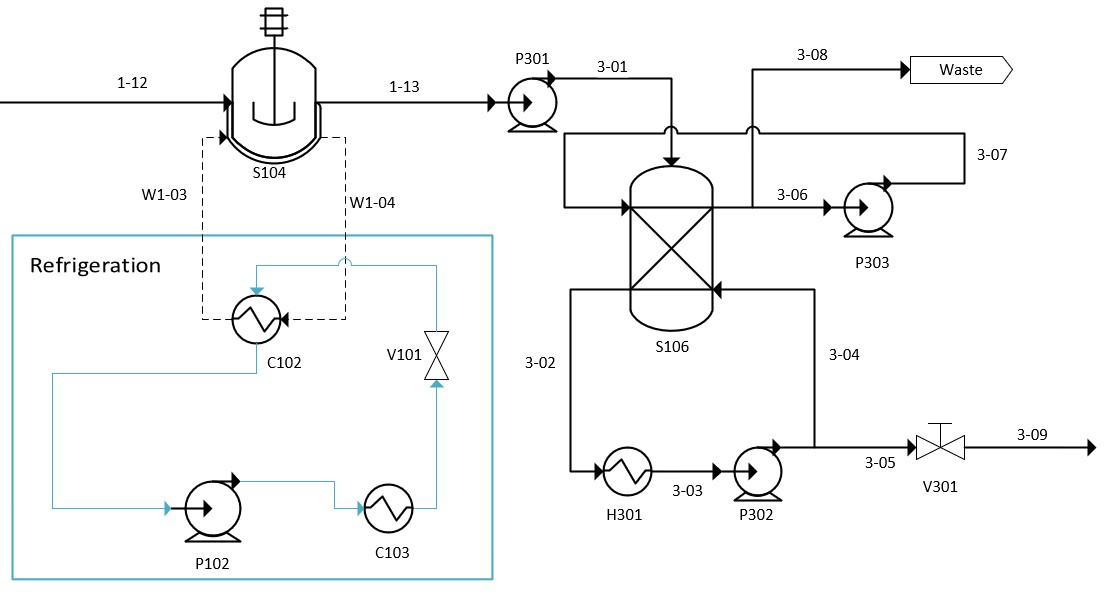
\includegraphics[scale=0.6]{chapters/3-separation/figures/Crystallizer PFD.jpg}
    \caption{PFD of the separation system in consideration; the system consists of a melt crystalliser (S104) and a subsequent hydraulic wash column (S106).}
    \label{fig:separator PFD}
\end{figure}